\chapter{Experiments}\label{ch:exp}

In this chapter,
we show experiments performed on genetic data.
That kind of data is usually high dimensional.
For this reason, the tools developed in the previous chapters are particularly suited to solve it.

\section{Setup}\label{sec:exp_setup}

\subsection{Genetic data}\label{subsec:genetic_data}

\footnote{
    Data available at \href{https://amp.pharm.mssm.edu/archs4/download.html}{this address},
    under the filename \texttt{human\_matrix.h5 v8}.
}

\begin{table}[!htb]
    \centering
    \setlength{\tabcolsep}{2pt}
    {\small
        \begin{tabular}{|c|c|c|}\hline
        \textbf{\# of samples} & \textbf{\# of features} & \textbf{N}\\ \hline
        $2\,695$ & $35\,238$  & $13$\\ \hline
        \end{tabular}
    }%
    \caption[short]{
        ARCHS4 dataset characteristics.
    }
    \label{tab:archs4_dataset}
\end{table}

\section{Results}\label{sec:exp_results}

\subsection{Applications}\label{subsec:nb_app}

The apparent low complexity of sparse naive Bayes compared to $\ell_1$-penalized methods such as
Lasso, logistic regression or SVMs makes is appealing for very large scale datasets.
We mention here a few applications to which we will come back later\footnote{
    An implementation of sparse naive Bayes can be found~\href{https://github.com/aspremon/NaiveFeatureSelection}{here}.
}.

\section{Criteo dataset}\label{sec:snb_criteo}

This experiments is not related to the knockoffs framework,
but shows the very good scalability of sparse naive Bayes presented in Section~\ref{sec:snb}.
As part of a Kaggle competition \emph{Display Advertising Challenge}\footnote{
    The Kaggle competition can be found at
    \href{https://www.kaggle.com/c/criteo-display-ad-challenge}{this address}.
}
in mid-2014, CriteoLabs shared log data collected over one week\footnote{
    The competition's dataset can be downloaded at
    \href{https://labs.criteo.com/2014/02/download-kaggle-display-advertising-challenge-dataset/}{this address}.
}
whose features were undisclosed for confidentiality purposes.
Main characteristics of this dataset can be found in Table~\ref{tab:criteo_dataset}.
\begin{table}[!htb]
    \centering
    \setlength{\tabcolsep}{2pt}
    {\small
        \begin{tabular}{|c|c|c|c|c|}\hline
        \textbf{Samples} & \textbf{Total features} & \textbf{Numerical features} & \textbf{Categorical features} & \textbf{Features after encoding}\\ \hline
        $45\,840\,617$ & $39$  & $13$ & $26$ & $33\,762\,590$ \\ \hline
        \end{tabular}
    }%
    \caption[short]{
        Criteo dataset characteristics.
        Even though the number of features is small,
        most categorical features have millions of categories.
        It makes the training of predicting models particularly challenging as it requires several
        dozens of GB of memory.
    }
    \label{tab:criteo_dataset}
\end{table}
It consists in $\approx 45$ millions of display ads with 39 features,
and a boolean label describing whether or not the ad was clicked by a customer.
Among these 39 features, 26 are categorical and a classical one-hot encoding would end up in millions of features.
This makes the Criteo dataset challenging, as it doesn't fit in the random-access memory after encoding,
and potentially not in the mass storage of a standard computer either.
Even on a small subset of the features, say 10\%,
selecting important features using Lasso or $\ell_1$-penalized logistic regression isn't realistic.
One-hot encoding isn't adapted to that situation.
Another approach would be to one-hot encode for each categorical feature only the most frequent categories,
and put the rest in a category \textit{other}.
The winners of the Kaggle competition used the hashing trick.
It consists in choosing an encoding space size $m$,
for example $m = 2^{20}$,
and defining some hash function $h \colon \text{Categories} \to \left\{ 0, \dots, m - 1 \right\}$.
This approach has several notable advantages.
First, the final encoded feature space $m$ can be adapted depending on the needs and on the computing power.
It may be used in an online fashion without a first pass
(that would be required for one-hot encoding in order to figure out all the existing categories).
Lastly, it naturally handles new labels in the test set that were unseen in the train set
(which would typically need a special \textit{other} category in the one-hot encoding setting).
Collisions between categories are likely to happen,
and even collisions between categories from different features.

We present here in Figure~\ref{fig:criteo_hash_elbow}.
$m = 2^{24} = 16777216$
All the computations are done on a standard workstation (16GB, Intel Core i7 3.60GHz $\times$ 8).
Sparse naive Bayes requires data averages to run,
i.e.\ the sums of the negative and of the positive points.
This part is time consuming but once these sums are computed they can be reused for any sparsity level $k$.
Using a light hash function and PyPy, they were obtained in around 20 minutes.
Only roughly half of the $2^{24}$ hash features were hit by the hash function.
Then, SNB optimum are computed for 1200 log-spaced points using a Python and NumPy implementation of SNB in 1 hour.
In this situation, what makes SNB particularly appealing is the fact that at no moment we need to load the full dataset
in memory.
We are only computing data averages whose shape are much smaller than the full matrix.
Note also that most tasks could even be distributed to speed up the computations.
\begin{figure}
    \centering
    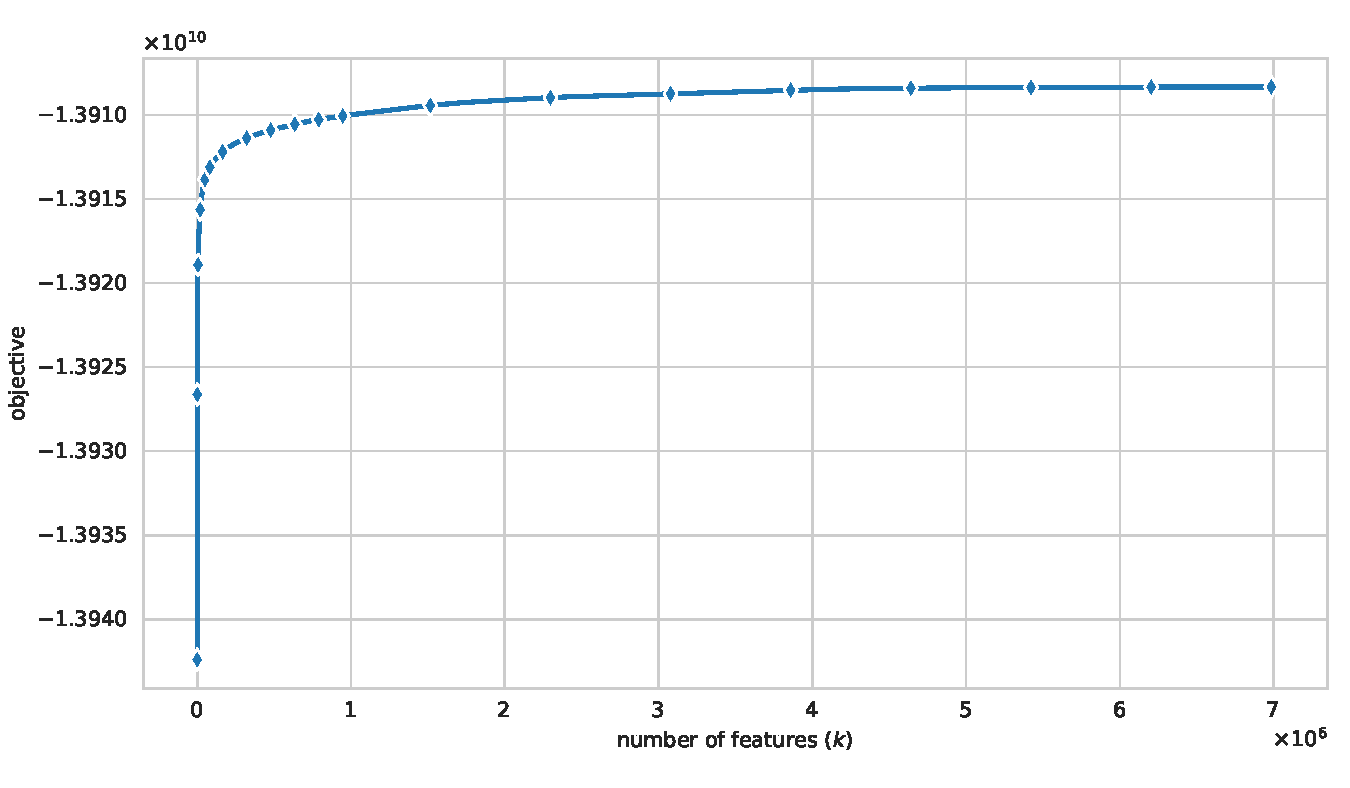
\includegraphics[width=0.75\linewidth, height=0.4\linewidth]{figures/criteo_hash_elbow.pdf}
    \caption{
        Optimal value of the~\ref{eq:msnb} optimization problem on the Criteo dataset
        as a function of the sparsity parameter $k$.
        Only 1--2 millions of the features explain most of the target vector (elbow heuristic).
    }
    \label{fig:criteo_hash_elbow}
\end{figure}

\subsubsection{Genetic and fMRI data}\label{subsubsec:snb_genetic_fmri}
